\chapter{Gabriel's Horn}

\begin{figure}[h]
    \centering
    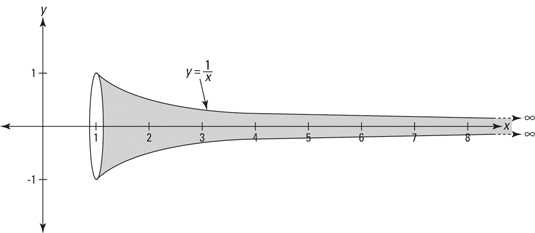
\includegraphics[width=3in]{assets/grabirels-horn.jpg}
    \caption{Gabriel's Horn}
\end{figure}

\noindent Finding the volume of Gabriel's Horn using the formula to find the volume of a solid of revolution:

\begin{align*}
V &= \pi \int_{1}^{\infty} \frac{1}{x^2} \, dx \\
  &= \pi \int_{1}^{\infty} x^{-2} \, dx \\
  &= \pi \left[-\frac{1}{x}\right]_{1}^{\infty} \\
  &= \pi \left(0 + 1\right) \\
  &= \pi
\end{align*}

\noindent Therefore, the volume of Gabriel's Horn is $\pi$.\\
\\Finding the surface area of Gabriel's Horn using the formula to find the surface area of a solid of revolution:

\begin{align*}
SA &= \int_{1}^{\infty} 2\pi \frac{1}{x} \sqrt{1+\left(-\frac{1}{x^2}\right)^2} \, dx \\
   &= 2\pi \int_{1}^{\infty} \frac{1}{x} \sqrt{1+\left(-\frac{1}{x^2}\right)^2} \, dx \\
   &= 2\pi \int_{1}^{\infty} \frac{1}{x} \sqrt{1+\frac{1}{x^4}} \, dx > 2\pi \int_{1}^{\infty} \frac{1}{x} \, dx \\ 
  &= \left[2\pi \ln |x|\right]_{1}^{\infty} \\
  &= 2\pi (\infty - 0) \\
SA &= \infty
\end{align*}

\noindent Since the integral does not converge, the surface area of Gabriel's Horn is infinite.
